
% xetex expected
\documentclass[xetex,professionalfont]{beamer}

% we want math
\usepackage{amsmath}

% fixes and extensions to amsmath
\usepackage{mathtools}

% additional math symbols
\usepackage{amssymb}

% good-looking fractions in text via \sfrac
\usepackage{xfrac}

% fix spaces after custom commands (see below for examples)
\usepackage{xspace}

% minted allows for fancy syntax highlighting (requires python with pygments)
% usage:
%   \begin{minted}{python}
%   codeb
%   \end{minted}
\usepackage{minted}

% better looking tables
% usage:
%   begin with a \toprule, write a single row of column headings,
%   then add \midrule and after the columns of data we finish with \bottomrule
% example:
%   \begin{tabular}{llr} \toprule
%   Animal & Description & Price \midrule
%   cat & foo & 10 \\
%   dog & bar & 20 \\ \bottomrule
%   \end{tabular}
% note that good tables generally neither have vertical rules nor double rules
\usepackage{booktabs}

% system font support (requires xetex or luatex)
\usepackage{fontspec}
\setmonofont[Scale=0.7]{Cousine} % part of ttf-chromeos fonts on Arch

% improve microtypography
\usepackage{microtype}

% multi-language quotes for babel
\usepackage{csquotes}

% easy way to include copyright information
\usepackage{copyrightbox}

% better bibliographies
\usepackage[backend=biber,style=authoryear]{biblatex}

% language support (english,ngerman)
\usepackage[english]{babel}

% process diagrams (part of texlive-pictures)
\usepackage{smartdiagram}

% plots
\usepackage{pgfplots}

% -----------------------------------------------------------------------------

% specify PDF metadata
\hypersetup{pdftitle={CVSP VO - Object Recognition 2 - Deep Learning},pdfsubject={},pdfauthor={Christopher Pramerdorfer}}

% copyright font style
\makeatletter\renewcommand{\CRB@setcopyrightfont}{\tiny\color{lightgray}}

% make emph bold
\DeclareTextFontCommand{\emph}{\bfseries}

% use proper fonts for math
% \usefonttheme[onlymath]{serif}

% use tuwcvl beamer theme
\usetheme{tuwcvl}

% add bib file
\addbibresource{literature.bib}

% diagram style

\smartdiagramset{norm/.style={
	 sequence item border color=gray!30!black,
	 sequence item border size=1.5\pgflinewidth,
	 sequence item font size=\footnotesize,
  }
}

\smartdiagramset{transp/.style={
	 sequence item border color=gray!70!black,
	 sequence item border size=1.5\pgflinewidth,
	 sequence item font size=\footnotesize,
	 sequence item fill opacity=0.5,
	 sequence item text opacity=0.5
  }
}

\smartdiagramset{norm}

% plot setup

\pgfplotsset{width=6.5cm,compat=newest}

\definecolor{darkgreen}{rgb}{0,0.8,0.1}

% -----------------------------------------------------------------------------

% common english abbreviations
\newcommand{\ie}{\mbox{i.e.}\xspace} % i.e.
\newcommand{\eg}{\mbox{e.g.}\xspace} % e.g.
\newcommand{\wrt}{\mbox{wrt.}\xspace} % wrt.

% math - argmin and argmax
\DeclareMathOperator*{\argmin}{arg\,min}
\DeclareMathOperator*{\argmax}{arg\,max}

% shortcuts for number ranges
\newcommand{\NN}{\mathbb{N}}
\newcommand{\ZZ}{\mathbb{Z}}
\newcommand{\QQ}{\mathbb{Q}}
\newcommand{\RR}{\mathbb{R}}

% bold vectors
\renewcommand{\vec}[1]{\ensuremath{\mathbf{#1}}}

% vector shortcuts
\newcommand{\va}{\vec{a}}
\newcommand{\vb}{\vec{b}}
\newcommand{\vc}{\vec{c}}
\newcommand{\ve}{\vec{e}}
\newcommand{\vr}{\vec{r}}
\newcommand{\vs}{\vec{s}}
\newcommand{\vt}{\vec{t}}
\newcommand{\vu}{\vec{u}}
\newcommand{\vv}{\vec{v}}
\newcommand{\vw}{\vec{w}}
\newcommand{\vx}{\vec{x}}
\newcommand{\vy}{\vec{y}}
\newcommand{\vz}{\vec{z}}

% -----------------------------------------------------------------------------

\title{Computer Vision Systems Programming VO}
\subtitle{Object Recognition -- Deep Learning}
\author{Christopher Pramerdorfer}
\institute{Computer Vision Lab, Vienna University of Technology}

\begin{document}

% disable minted's syntax checks
\expandafter\def\csname PY@tok@err\endcsname{}

% -----------------------------------------------------------------------------

\begin{frame}
\maketitle
\end{frame}

% -----------------------------------------------------------------------------

\begin{frame}
\frametitle{Topics}

Deep learning motivation\\\medskip
Multilayer perceptrons\\\medskip
Convolutional neural networks\\\medskip
Deep learning applications

\bigskip
\begin{center}
	\copyrightbox[b]
	{\includegraphics[width=10cm]{figures/intro-collage.png}}
	{\centering Images from \cite{lecun1989}, \cite{taigman2013}, \url{image-net.org}}
\end{center}

\end{frame}

% -----------------------------------------------------------------------------

\begin{frame}
\frametitle{Object Recognition}
\framesubtitle{Traditional Approach}

\begin{center}
\smartdiagram[sequence diagram]{Image,Feature Extraction,Learned Mapping}\\\bigskip % learned mapping maps from the representation to the output, such as a class label, i.e. this is our model. however, in this context we don't really know the relation between features and classes (there is no clear relation between the information we are interested in an the measurements, in contrast to e.g. structure from motion), so we use some general model like an SVM, for example.
\smartdiagramset{transp}
\smartdiagram[sequence diagram]{Image,SIFT+BOW,SVM} % this is the bag of visual words based image classification method we covered in the previous lecture
\end{center}

\end{frame}

% -----------------------------------------------------------------------------

\begin{frame}
\frametitle{Object Recognition}
\framesubtitle{Traditional Approach}

Problem: how to choose the representation/features? % the representation comprises all features, for example the visual word frequencies in case of bag of visual words

\bigskip
\enquote{General} features not optimal % like sift or others
\begin{itemize}
	\item Not tuned to task at hand, low-level
\end{itemize}

\bigskip
Designing task-specific features is complex
\begin{itemize}
	\item Virtually impossible to do optimally % think of manually designing features that respond to human heads (not a single one, but to heads in general)
\end{itemize}

\end{frame}

% -----------------------------------------------------------------------------

\begin{frame}
\frametitle{Object Recognition}
\framesubtitle{Deep Learning}

Solution: learn representation as well\\\medskip % this is called ... representation learning
Learning high-level representations directly is difficult

\bigskip
\emph{Deep Learning} (DL) solves this
\begin{itemize}
	\item By learning a hierarchy of representations % hence "deep" / hierarchy is fixed, everything else is learned
	\item Layers in hierarchy build upon each other % from low-level to high-level representation
\end{itemize}

\end{frame}

% -----------------------------------------------------------------------------

\begin{frame}
\frametitle{Object Recognition}
\framesubtitle{Deep Learning}

\begin{center}
	\copyrightbox[b]
	{\includegraphics[width=7.5cm]{figures/dl-layer-example.png}}
	{\centering Image from \cite{bengio2014}}
\end{center}

\end{frame}

% -----------------------------------------------------------------------------

\begin{frame}
\frametitle{Object Recognition}
\framesubtitle{Deep Learning}

$n$ levels of features/representations\\\medskip
Learned jointly with the output mapping

\bigskip
\begin{center}
\smartdiagramset{sequence item text width=1cm}
\smartdiagram[sequence diagram]{Image,LF $1$,$\dots$,LF $n$,LM} % LF = learned features, % LM = learned mapping
\end{center}

\end{frame}

% -----------------------------------------------------------------------------

\begin{frame}
\frametitle{Object Recognition}
\framesubtitle{Deep Learning}

Methods based on DL are state of the art
\begin{itemize}
	\item For almost all recognition-related CV tasks
\end{itemize}

\bigskip
\begin{center}
	\enquote{From now on, DL has to be considered as the primary\\ candidate in essentially any visual recognition task}\\
	~ [\cite{razavian14}] % check out this paper. also see Pierre Sermanet's slides for a good overview of how DL has advanced the state of the art in many fields, available here: https://sites.google.com/site/deeplearningcvpr2014/
\end{center}

\end{frame}

% -----------------------------------------------------------------------------

\begin{frame}
\frametitle{Multilayer Perceptrons}

DL is realized using MultiLayer Perceptrons (MLPs) % also known as feed-forward neural networks

\bigskip
\begin{center}
	\copyrightbox[b]
	{\includegraphics[width=4.5cm]{figures/two-layer-mlp.png}}
	{\centering Image from \cite{bishop2006}}
\end{center}

\end{frame}

% -----------------------------------------------------------------------------

\begin{frame}
\frametitle{Multilayer Perceptrons}
\framesubtitle{The Perceptron}

Binary linear classifier\\\medskip
Feature vectors $\vx$ classified as $f(\vw^\top\vx+b)\in\{-1,+1\}$\\\medskip % sometimes {0,1} is used, but {-1,1} facilitates training
$f$ is a discontinuous step function % so f is not differentiable
\[
f(v)=\begin{cases}
	+1 & \text{if } v>0\\
	-1 & \text{otherwise}
\end{cases}
\]\\\medskip
$\vw,b$ learned from training data % the decision hyperplane is wx+b=0

\end{frame}

% -----------------------------------------------------------------------------

\begin{frame}
\frametitle{Multilayer Perceptrons}
\framesubtitle{The Perceptron}

\begin{center}
	\includegraphics[width=7cm]{figures/perceptron-classification.pdf} % see code/perceptron.py
\end{center}

\end{frame}

% -----------------------------------------------------------------------------

\begin{frame}
\frametitle{Multilayer Perceptrons}
\framesubtitle{The Perceptron -- Limitations}

Only two classes\\\medskip % but there are extension to multiple classes
Linear decision boundaries\\\medskip % and these are not optimal in terms of margin, as opposed to SVM (but this applies to the MLP as well)
Learning never converges for non-separable data % so if we don't know whether our training data is linearly separable, we are in trouble

\end{frame}

% -----------------------------------------------------------------------------

\begin{frame}
\frametitle{Multilayer Perceptrons}
\framesubtitle{Two-Layer Architecture}

% here we only cover the standard two-layer architecture, which is the most common for "traditional MLPs" as they can encode any continuous decision boundary, as long as the number of hidden units is large enough. however, the architecture can be arbitrary as long as all nonlinearities are differentiable and there are no closed directed cycles in the graph

Replace $f$ with continuous nonlinearity (\eg $\tanh(\cdot)$)\\\medskip % differentiable
Introduce layer of $M$ such \enquote{Perceptrons} (hidden units)\\\medskip % no longer perceptrons but logistic regression models after replacing f, hence the quotes
Hidden units connected to layer of $K$ output units

\begin{center}
	\copyrightbox[b]
	{\includegraphics[width=4.5cm]{figures/two-layer-mlp.png}}
	{\centering Image from \cite{bishop2006}}
\end{center}

\end{frame}

% -----------------------------------------------------------------------------

\begin{frame}
\frametitle{Multilayer Perceptrons}
\framesubtitle{Two-Layer Architecture}

Output of $m$th hidden unit is $z_m(\vx)=f(\vw_m^\top\vx)$
\begin{itemize}
	\item Bias $b$ included in $\vw$ and $\vx$, $w_0=b$, $x_0=1$
\end{itemize}

\bigskip
\begin{center}
	\copyrightbox[b]
	{\includegraphics[width=4.5cm]{figures/two-layer-mlp.png}}
	{\centering Image from \cite{bishop2006}}
\end{center}

\end{frame}

% -----------------------------------------------------------------------------

\begin{frame}
\frametitle{Multilayer Perceptrons}
\framesubtitle{Two-Layer Architecture}

Output of $k$th output unit is $y_k(\vz)=g(\vw_k^\top\vz)$\\\medskip % this again includes the bias
Choice of $g$ depends on problem (regression, classification) % identity for regression, softmax for classification; must be differentiable

\bigskip
\begin{center}
	\copyrightbox[b]
	{\includegraphics[width=4.5cm]{figures/two-layer-mlp.png}}
	{\centering Image from \cite{bishop2006}}
\end{center}

\end{frame}

% -----------------------------------------------------------------------------

\begin{frame}
\frametitle{Multilayer Perceptrons}
\framesubtitle{Two-Layer Architecture}

Both $f$ and $g$ are differentiable
\begin{itemize}
	\item Learn $\vw$ using gradient descent % here w contains all weights / the error function to minimize depends on the task; for regression we minimize the sum of squared residuals
	\item Gradients evaluated via error backpropagation % no details here, check bishop2006, for example
\end{itemize}

\end{frame}

% -----------------------------------------------------------------------------

\begin{frame}
\frametitle{The Pylearn2 Library}

Machine learning library with focus on DL\\\medskip
Written in Python, but interaction mostly in YAML\\\medskip
Open-source: \url{https://github.com/lisa-lab/pylearn2}

\end{frame}

% -----------------------------------------------------------------------------

\begin{frame}
\frametitle{The Pylearn2 Library}
\framesubtitle{MLP Regression Example}

Use pylearn2 to train a MLP for regression

\medskip
\begin{center}
	\includegraphics[width=6cm]{figures/mlp-input.pdf} % see code/mlp_gen_data_regression.py
\end{center}

\end{frame}

% -----------------------------------------------------------------------------

\begin{frame}[fragile]
\frametitle{The Pylearn2 Library}
\framesubtitle{MLP Regression Example}

% irange means "init weights randomly from [-irange,+irange]"
% linear layer means g() = identity

\begin{minted}[fontsize=\footnotesize]{yaml}
model: !obj:pylearn2.models.mlp.MLP {
    nvis: 1, # one input unit x
    layers: [ # two layers
        !obj:pylearn2.models.mlp.Tanh { # tanh activations for hidden units
            dim: 3, # use M=3 hidden units
            layer_name: 'hidden',
            irange: 0.1
        },
        !obj:pylearn2.models.mlp.Linear { # linear output layer for regression
            dim: 1, # one output unit, K=1 
            layer_name: 'out',
            irange: 0.1
        }
    ]
}
\end{minted}

\end{frame}

% -----------------------------------------------------------------------------

% see code/mlp_regression.yaml for the full code

\begin{frame}[fragile]
\frametitle{The Pylearn2 Library}
\framesubtitle{MLP Regression Example}

\begin{minted}[fontsize=\footnotesize]{yaml}
# dataset contains the (x,y) pairs from the previous figure
dataset: &train !pkl: 'mlp_data_regression.pkl',
# train using batch gradient descent
algorithm: !obj:pylearn2.training_algorithms.bgd.BGD {
    conjugate: 1,
    batch_size: 50,
    line_search_mode: 'exhaustive',
    termination_criterion: !obj:pylearn2.termination_criteria.EpochCounter {
        max_epochs: 100 # train for 100 epochs
    }
}
\end{minted}

\end{frame}

% -----------------------------------------------------------------------------

\begin{frame}
\frametitle{The Pylearn2 Library}
\framesubtitle{MLP Regression Example}

Full example: \url{https://github.com/cpra/cvsp-vo-slides}

\medskip
\begin{center}
	\includegraphics[width=6cm]{figures/mlp-regression.pdf} % see code/mlp_test_data_regression.py ... we would get a perfect fit if we trained longer
\end{center}

\end{frame}

% -----------------------------------------------------------------------------

\begin{frame}
\frametitle{Convolutional Neural Networks}
\framesubtitle{Motivation}

Above MLP architecture does not scale to images
\begin{itemize}
    \item VGA resolution, $M=1000$: $\sim300$ million params % we don't have enough images to train such nets without running into overfitting problems. also, such models are too general in an image context, because they do not enforce constraints due to the topology of images (adjacent pixels are correlated because they correspond to adjacent parts of the depicted object)
\end{itemize}

\medskip
\begin{center}
\begin{tikzpicture}
\node [inner sep=0pt,above right]{\includegraphics[width=4cm]{figures/blue-mosque.jpg}};
\draw[step=1mm, black] (0,0) grid (4,3);
\foreach \m in {0.5,1.5,2.5} {
    \foreach \x in {0.05,0.45,...,3.95} {
        \foreach \y in {0.05,0.45,...,2.95} {
            \draw[black,opacity=0.33] (\x,\y) -- (7, \m);
        }
    }
    \draw[blue,thick,fill=white] (7,\m) circle (0.05cm);
}
\end{tikzpicture}
\end{center}

\end{frame}

% -----------------------------------------------------------------------------

\begin{frame}
\frametitle{Convolutional Neural Networks}
\framesubtitle{Motivation}

% i'm using red, green, blue here without relating to RGB image channels

Nearby pixels are closely correlated\\\medskip % this is why local features work ... in fact what the resulting hidden units learn are distinctive local features
Exploit topology through locally connected layers % this concept is called local receptive fields

\medskip
\begin{center}
\begin{tikzpicture}
\node [inner sep=0pt,above right]{\includegraphics[width=4cm]{figures/blue-mosque.jpg}};
\draw[step=1mm, black] (0,0) grid (0.5,0.5);
\draw[thick,red] (0,0) rectangle (0.5,0.5);
\foreach \x in {0.05,0.15,...,0.45} {
    \foreach \y in {0.05,0.15,...,0.45} {
        \draw[red,opacity=0.33] (\x,\y) -- (7, 0.25);
    }
}
\draw[step=1mm, black] (1,1) grid (1.5,1.5);
\draw[thick,darkgreen] (1,1) rectangle (1.5,1.5);
\foreach \x in {1.05,1.15,...,1.45} {
    \foreach \y in {1.05,1.15,...,1.45} {
        \draw[darkgreen,opacity=0.33] (\x,\y) -- (7, 1.25);
    }
}
\draw[step=1mm, black] (2,2) grid (2.5,2.5);
\draw[thick,blue] (2,2) rectangle (2.5,2.5);
\foreach \x in {2.05,2.15,...,2.45} {
    \foreach \y in {2.05,2.15,...,2.45} {
        \draw[blue,opacity=0.33] (\x,\y) -- (7, 2.25);
    }
}
\draw[blue,thick,fill=white] (7,0.25) circle (0.05cm);
\draw[blue,thick,fill=white] (7,1.25) circle (0.05cm);
\draw[blue,thick,fill=white] (7,2.25) circle (0.05cm);
\end{tikzpicture}
\end{center}

\end{frame}

% -----------------------------------------------------------------------------

\begin{frame}
\frametitle{Convolutional Neural Networks}
\framesubtitle{Convolutional Layers}

Convolutional layer consists of $F$ feature maps\\\medskip % which usually have the same size as the input, as shown in the image
Each map consists of $M$ hidden units with \emph{shared} weights\\\medskip % the motivation for this is that features that are useful in one region in the image should be so also in other regions ... by this we gain translation invariance
Hidden units have a local receptive field % i.e. connected to only a local neighborhood in the input layer (the image in the below figure). this is motivated by the correlation characteristics outlined above

% as all units have a local receptive field and because the weights are shared, the transformations carried out by a feature map (before applying the nonlinearity) corresponds to a convolution with a learned kernel w, hence convolutional NN

\medskip
\begin{center}
\begin{tikzpicture}
\node [inner sep=0pt,above right]{\includegraphics[width=4cm]{figures/blue-mosque.jpg}};;
\draw[step=1mm, black] (2,2) grid (2.5,2.5);
\draw[thick,blue] (2,2) rectangle (2.5,2.5);
\foreach \x in {2.05,2.15,...,2.45} {
    \foreach \y in {2.05,2.15,...,2.45} {
        \draw[darkgreen,opacity=0.33] (\x,\y) -- (7.65, 2.65);
        \draw[red,opacity=0.33] (\x,\y) -- (7.45, 2.45);
        \draw[blue,opacity=0.33] (\x,\y) -- (7.25, 2.25);
    }
}
\draw[step=1mm,darkgreen,opacity=0.33] (5.4,0.4) grid (9.4,3.4);
\draw[darkgreen] (5.4,0.4) rectangle (9.4,3.4);
%
\draw[step=1mm,red,opacity=0.33] (5.2,0.2) grid (9.2,3.2);
\draw[red] (5.2,0.2) rectangle (9.2,3.2);
%
\draw[step=1mm,blue,opacity=0.33] (5,0) grid (9,3);
\draw[blue] (5,0) rectangle (9,3);
%
\draw[draw=none,fill=darkgreen] (7.6,2.6) rectangle (7.7,2.7);
\draw[draw=none,fill=red] (7.4,2.4) rectangle (7.5,2.5);
\draw[draw=none,fill=blue] (7.2,2.2) rectangle (7.3,2.3);
%
\node at (9.25,0) {\footnotesize $1$};
\node at (9.5,0.25) {\footnotesize $\;\dots$};
\node at (9.75,0.5) {\footnotesize $F$};
\end{tikzpicture}
\end{center}

\end{frame}

% -----------------------------------------------------------------------------

\begin{frame}
\frametitle{Convolutional Neural Networks}
\framesubtitle{Convolutional Layers}

% note that the activations f are usually not tanh but max(0,.). such units are called maxout units or rectified linear units (ReLUs). using maxout can make training several times faster (see Krizhevsky12) ... but there are other possibilities as well, such as |x|

Number of params independent of image resolution and $M$\\\medskip
$F=100$, $15\times15$ receptive field: $\sim23,000$ params

\bigskip
Feature map evaluation equals
\begin{itemize}
    \item Convolution with kernel $\vw_f$ (hence the name) % because of the shared weights
    \item Followed by nonlinearity $f(\cdot)=\max(0,\cdot)$ (ReLU) % see above
\end{itemize}

\medskip
\begin{center}
    \copyrightbox[b]
    {\includegraphics[width=5cm]{figures/learned-kernels.png}} % image shows trained weights, which have a typical appearance (most are Gabor-like)
    {\centering Image from \cite{krizhevsky2012}}
\end{center}

\end{frame}

% -----------------------------------------------------------------------------

\begin{frame}
\frametitle{Convolutional Neural Networks}
\framesubtitle{Pooling Layers}

After convolutional layer\\\medskip
Hidden units pool information locally (\eg max, avg)\\\medskip % usually it's max
Data reduction, robustness to small translations % of the input images

% the below figure shows a 2x2 pooling layer, which is a common size
% pooling layers have no nonlinearity, but sometimes trained weights

\medskip
\begin{center}
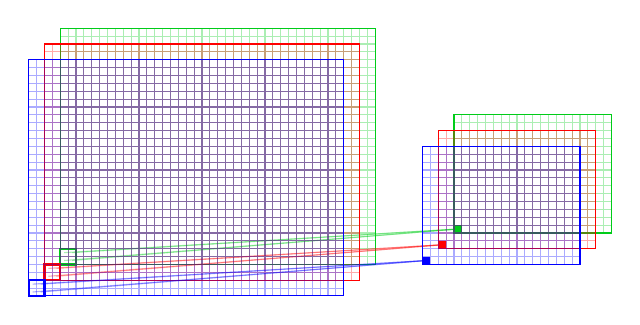
\begin{tikzpicture}
% green
\draw[step=1mm,darkgreen,opacity=0.33] (0.4,0.4) grid (4.4,3.4);
\draw[darkgreen] (0.4,0.4) rectangle (4.4,3.4);
%
\draw[step=1mm,darkgreen,opacity=0.33] (5.4,0.8) grid (7.4,2.3);
\draw[darkgreen] (5.4,0.8) rectangle (7.4,2.3);
%
\draw[darkgreen,thick] (0.4,0.4) rectangle (0.6,0.6);
\draw[draw=none,fill=darkgreen] (5.4,0.8) rectangle (5.5,0.9);
\draw[darkgreen,opacity=0.33] (0.45,0.45) -- (5.45, 0.85);
\draw[darkgreen,opacity=0.33] (0.55,0.45) -- (5.45, 0.85);
\draw[darkgreen,opacity=0.33] (0.45,0.55) -- (5.45, 0.85);
\draw[darkgreen,opacity=0.33] (0.55,0.55) -- (5.45, 0.85);
%
% red
%
\draw[step=1mm,red,opacity=0.33] (0.2,0.2) grid (4.2,3.2);
\draw[red] (0.2,0.2) rectangle (4.2,3.2);
%
\draw[step=1mm,red,opacity=0.33] (5.2,0.6) grid (7.2,2.1);
\draw[red] (5.2,0.6) rectangle (7.2,2.1);
%
\draw[red,thick] (0.2,0.2) rectangle (0.4,0.4);
\draw[draw=none,fill=red] (5.2,0.6) rectangle (5.3,0.7);
\draw[red,opacity=0.33] (0.25,0.25) -- (5.25, 0.65);
\draw[red,opacity=0.33] (0.35,0.25) -- (5.25, 0.65);
\draw[red,opacity=0.33] (0.25,0.35) -- (5.25, 0.65);
\draw[red,opacity=0.33] (0.35,0.35) -- (5.25, 0.65);
%
% blue
%
\draw[step=1mm,blue,opacity=0.33] (0,0) grid (4,3);
\draw[blue] (0,0) rectangle (4,3);
%
\draw[step=1mm,blue,opacity=0.33] (5,0.4) grid (7,1.9);
\draw[blue] (5,0.4) rectangle (7,1.9);
%
\draw[blue,thick] (0,0) rectangle (0.2,0.2);
\draw[draw=none,fill=blue] (5,0.4) rectangle (5.1,0.5);
\draw[blue,opacity=0.33] (0.05,0.05) -- (5.05, 0.45);
\draw[blue,opacity=0.33] (0.15,0.05) -- (5.05, 0.45);
\draw[blue,opacity=0.33] (0.05,0.15) -- (5.05, 0.45);
\draw[blue,opacity=0.33] (0.15,0.15) -- (5.05, 0.45);
\end{tikzpicture}
\end{center}

\end{frame}

% -----------------------------------------------------------------------------

\begin{frame}
\frametitle{Convolutional Neural Networks}
\framesubtitle{Local Contrast Normalization Layers}

% such layers have neither nonlinearities nor trained weights (only a couple hyperparameters)

Between convolution and pooling layers\\\medskip
Normalize responses spatially or over adjacent feature maps\\\medskip % below image shows normalization across maps
Produce more expressive, robust features

\medskip
\begin{center}
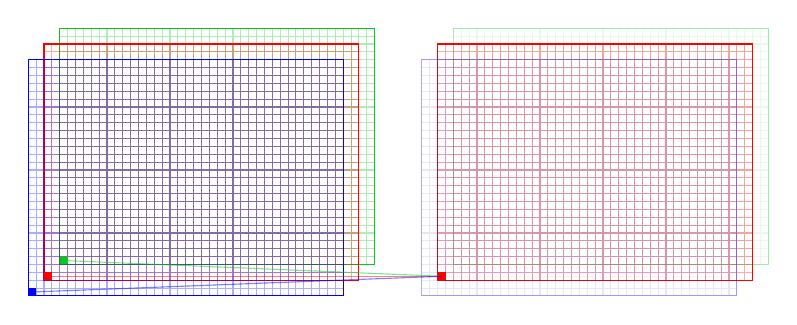
\begin{tikzpicture}
% green
\draw[step=1mm,darkgreen,opacity=0.33] (0.4,0.4) grid (4.4,3.4);
\draw[darkgreen] (0.4,0.4) rectangle (4.4,3.4);
\draw[step=1mm,darkgreen,opacity=0.1] (5.4,0.4) grid (9.4,3.4);
\draw[darkgreen,opacity=0.33] (5.4,0.4) rectangle (9.4,3.4);
% red
\draw[step=1mm,red,opacity=0.33] (0.2,0.2) grid (4.2,3.2);
\draw[red] (0.2,0.2) rectangle (4.2,3.2);
\draw[step=1mm,red,opacity=0.33] (5.2,0.2) grid (9.2,3.2);
\draw[red] (5.2,0.2) rectangle (9.2,3.2);
% blue
\draw[step=1mm,blue,opacity=0.33] (0,0) grid (4,3);
\draw[blue] (0,0) rectangle (4,3);
\draw[step=1mm,blue,opacity=0.1] (5,0) grid (9,3);
\draw[blue,opacity=0.33] (5,0) rectangle (9,3);
% units
\draw[draw=none,fill=darkgreen] (0.4,0.4) rectangle (0.5,0.5);
\draw[draw=none,fill=red] (0.2,0.2) rectangle (0.3,0.3);
\draw[draw=none,fill=blue] (0,0) rectangle (0.1,0.1);
\draw[draw=none,fill=red] (5.2,0.2) rectangle (5.3,0.3);
% lines
\draw[darkgreen,opacity=0.5] (0.45,0.45) -- (5.25, 0.25);
\draw[red,opacity=0.5] (0.25,0.25) -- (5.25, 0.25);
\draw[blue,opacity=0.5] (0.05,0.05) -- (5.25, 0.25);
\end{tikzpicture}
\end{center}

\end{frame}

% -----------------------------------------------------------------------------

\begin{frame}
\frametitle{Convolutional Neural Networks}
\framesubtitle{Architecture}

% details vary strongly depending on the task at hand, of course

MLPs with above layers are Convolutional Neural Networks (CNNs)\\\medskip
Usually several Conv $\Rightarrow$ Norm $\Rightarrow$ Pooling blocks\\\medskip
Later Conv layers operate on multiple feature maps % i.e. they have a 3D receptive field / correspond to 3D convolutions (like 5x5x10 = 5x5 over 10 feature maps)

\medskip
\begin{center}
    \copyrightbox[b]
    {\includegraphics[width=8cm]{figures/cnp-layers.png}}
    {\centering Image adapted from \cite{kavukcuoglu2011}}
\end{center}

\end{frame}

% -----------------------------------------------------------------------------

\begin{frame}
\frametitle{Convolutional Neural Networks}
\framesubtitle{Architecture}

Blocks followed by a traditional MLP

\bigskip
\begin{center}
    \copyrightbox[b]
    {\includegraphics[width=9cm]{figures/convnet.pdf}}
    {\centering Image adapted from \cite{sermanet2012}} % this net is a bit more complicated because it has skip connections
\end{center}

\end{frame}

% -----------------------------------------------------------------------------

\begin{frame}
\frametitle{Deep Learning Applications}
\framesubtitle{Zip Code Recognition}

Zip code recognition from images\\\medskip
Among first applications of CNNs (1989!)
\begin{itemize}
    \item DL and CNNs are \enquote{old} concepts
    \item Now successful due to available data \& processing power % of course stuff has changed since then, like better nonlinearities, architectures, training methods
\end{itemize}

\bigskip
\begin{center}
    \copyrightbox[b]
    {\includegraphics[width=4cm]{figures/zip-numbers.png}}
    {\centering Image from \cite{lecun1989}}
\end{center}

\end{frame}

% -----------------------------------------------------------------------------

\begin{frame}
\frametitle{Deep Learning Applications}
\framesubtitle{Zip Code Recognition}

% H1: convolutional with 5x5 receptive field, 12 feature maps, 2x2 pooling (during convolution, to be precise ... see the paper for more information), also, biases as not shared in this case
% H2: 5x5x8 receptive field (see above slide), 12 feature maps, 2x2 pooling as above
% H3: hidden layer of traditional MLP with H2 as input
% total number of params is only around 10k

\begin{center}
    \copyrightbox[b]
    {\includegraphics[width=6.5cm]{figures/zip-dnn.png}}
    {\centering Image from \cite{lecun1989}}
\end{center}

\end{frame}

% -----------------------------------------------------------------------------

\begin{frame}
\frametitle{Deep Learning Applications}
\framesubtitle{Zip Code Recognition}

Let's try this ourselves\\\medskip
\url{http://cs.stanford.edu/people/karpathy/convnetjs/demo/mnist.html}

\bigskip
\begin{center}
    \copyrightbox[b]
    {\includegraphics[width=5cm]{figures/convnetjs-logo.png}}
    {\centering Image from \url{convnetjs.com}}
\end{center}

\end{frame}

% -----------------------------------------------------------------------------

\begin{frame}
\frametitle{Deep Learning Applications}
\framesubtitle{Face Recognition}

Large market (expected $\$6.5$B by 2018) % http://www.marketsandmarkets.com/PressReleases/facial-recognition.asp
\begin{itemize}
    \item Security, law enforcement, HCI, ...
\end{itemize}

\bigskip
Complicated task
\begin{itemize}
    \item Pose, occlusions, aging, expressions, accessories
\end{itemize}

\bigskip
\begin{center}
    \copyrightbox[b]
    {\includegraphics[width=7cm]{figures/lfw.png}}
    {\centering Image adapted from \url{http://vis-www.cs.umass.edu/lfw/}}
\end{center}

\end{frame}

% -----------------------------------------------------------------------------

\begin{frame}
\frametitle{Deep Learning Applications}
\framesubtitle{Face Recognition -- \cite{taigman2013}}

Face recognition via 3D face frontalization and DL
\begin{itemize}
    \item Conv $\Rightarrow$ Pooling $\Rightarrow$ Conv for low-level features
    \item Locally connected layers for high-level features % these are conv layers without weight sharing, hence the large number of parameters. weight sharing is not used here because features differ between face regions (faces are aligned)
    \item $\sim120$ million parameters, $~\sim4$ million training images
\end{itemize}

\bigskip
\begin{center}
    \copyrightbox[b]
    {\includegraphics[width=10cm]{figures/deepface-net.jpg}}
    {\centering Image from \cite{taigman2013}}
\end{center}

\end{frame}

% -----------------------------------------------------------------------------

\begin{frame}
\frametitle{Deep Learning Applications}
\framesubtitle{Face Recognition -- \cite{taigman2013}}

Human-level face verification performance % verification is 1:1, do two images depict the same person? see the below tech report for open and closed set classification results

\bigskip
\begin{center}
    \copyrightbox[b]
    {\includegraphics[width=5.5cm]{figures/fv-performance.png}} % some more recent improvements surpass human performance, see "Web-scale training for face identification" by Taigman et al.
    {\centering Image from \cite{taigman2013}}
\end{center}

\end{frame}

% -----------------------------------------------------------------------------

\begin{frame}
\frametitle{Deep Learning Applications}
\framesubtitle{Object Recognition}

Object recognition on the ImageNet database
\begin{itemize}
    \item $\sim14$ million images categorized hierarchically
    \item Annual object recognition challenges
\end{itemize}

\begin{center}
    \copyrightbox[b]
    {\includegraphics[width=8cm]{figures/imagenet.jpg}}
    {\centering Image from \url{http://web.eecs.umich.edu/~jiadeng/}}
\end{center}

\end{frame}

% -----------------------------------------------------------------------------

\begin{frame}[fragile]
\frametitle{Deep Learning Applications}
\framesubtitle{Object Recognition}

DL has lead to significant performance gains on ImageNet

% check the website for more infos on the newest results and the DL architectures used
% basically it's smaller receptive fields and deeper architectures (up to 19 in case of the 2014 runner up, for around 140 million parameters)

% below errors are top-5 error percentages - result is regarded as correct if one out of five reported categories corresponds to the true label (because there are multiple objects in the images, causing ambiguity) in case of classification. for localization, the bounding box must be correct as well.

\bigskip
\begin{center}
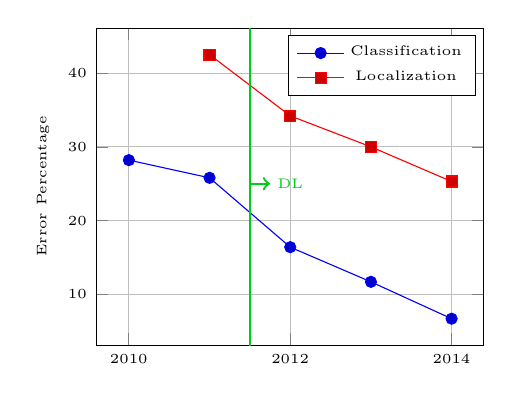
\begin{tikzpicture}
\begin{axis}[
    x tick label style={/pgf/number format/1000 sep=},
    ylabel=Error Percentage,
    font=\tiny,
    ylabel near ticks,
    grid=major
]
\addplot coordinates {(2010,28.2) (2011,25.8) (2012,16.4) (2013,11.7) (2014,6.7)};
\addplot coordinates {(2011,42.5) (2012,34.2) (2013,30.0) (2014,25.3)};
\draw [darkgreen,thick] (axis cs:2011.5,0) -- (axis cs:2011.5,50);
\draw [->,darkgreen,thick] (axis cs:2011.5,25) -- (axis cs:2011.75,25);
\node [darkgreen,thick] at (axis cs:2012,25) {DL};
\legend{Classification,Localization}
\end{axis}
\end{tikzpicture}
\end{center}

\end{frame}

% -----------------------------------------------------------------------------

\begin{frame}[fragile]
\frametitle{Deep Learning Applications}
\framesubtitle{Object Recognition}

Results of 2014 ImageNet object detection challenge (excerpt) % see below slide for detection definition

% DL wins if there is much data available (no *), but a shallow method MUS won the competition on a reduced data set (*) to a deep method (MSRA). complex DL nets require a significant amount of training data due to the large number of parameters, which can be a limitation

\begin{center}
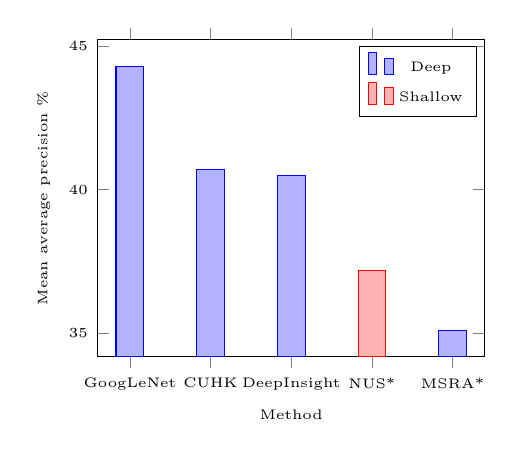
\begin{tikzpicture}
\begin{axis}[
    symbolic x coords={GoogLeNet,CUHK,DeepInsight,NUS*,MSRA*},
    xtick={GoogLeNet,CUHK,DeepInsight,NUS*,MSRA*},
    ybar,
    bar shift=0pt,
    font=\tiny,
    xlabel=Method,
    ylabel=Mean average precision \%
]
\addplot coordinates {(GoogLeNet,44.3) (CUHK,40.7) (DeepInsight,40.5) (MSRA*,35.11)};
\addplot coordinates {(NUS*,37.2)};
\legend{Deep,Shallow}
\end{axis}
\end{tikzpicture}
\end{center}

\end{frame}

% -----------------------------------------------------------------------------

\begin{frame}
\frametitle{Deep Learning Applications}
\framesubtitle{Object Recognition -- \cite{krizhevsky2012}}

Object classification and localization via DL\\\medskip % classification: assign single label of the main object present in the image / localization: do the same, but also locate it in the image. detection would be to locate any number of objects (including zero), and segmentation involves labeling each pixel
Won the 2012 challenge by a large margin\\\medskip % 10% better classification, 15% better localization
$\sim60$ million parameters, $\sim1.2$ million training images % training took 5-6 days on two GPUs

\bigskip
\begin{center}
\smartdiagramset{sequence item text width=0.8cm,sequence item width=1.25cm}
\smartdiagram[sequence diagram]{CNP,CNP,CCC,P,FF}
\end{center}

\end{frame}

% -----------------------------------------------------------------------------

\begin{frame}
\frametitle{Deep Learning Applications}
\framesubtitle{Object Recognition -- \cite{krizhevsky2012}}

Implemented using cuda-convnet
\begin{itemize}
    \item \url{https://code.google.com/p/cuda-convnet/}
    \item Open-source C++/CUDA implementation of CNNs
    \item Network structure definitions available on the webpage
\end{itemize}

\end{frame}

% -----------------------------------------------------------------------------

\begin{frame}
\frametitle{Deep Learning Applications}
\framesubtitle{Object Recognition}

\begin{center}
    Online demo of 2013 winner of classification challenge

    \bigskip
    \url{http://www.clarifai.com/}
\end{center}

\end{frame}

% -----------------------------------------------------------------------------

\begin{frame}
\frametitle{Deep Learning Applications}
\framesubtitle{Other Applications}

Scene labeling\\\medskip
Action recognition\\\medskip
Speech recognition\\\medskip
...

% see Sermannet's slides, link is above
% video of pedestrian detection: https://www.youtube.com/watch?v=uKU2pzpGUlM

\end{frame}

% -----------------------------------------------------------------------------

\begin{frame}
\frametitle{Remarks}

DL and CNNs are very powerful concepts
\begin{itemize}
    \item State of the art results in many areas of application
\end{itemize}

\bigskip
Training CNNs is complex
\begin{itemize}
    \item Some CNNs are trained on GPUs for weeks
    \item Large training datasets required % there are methods to compensate for this need to some degree, like data transformations, unsupervised pretraining, transfer learning ... check the literature
    \item Reason why DL became popular only recently
\end{itemize}

\bigskip
Several free implementations available
\begin{itemize}
    \item pylearn2, convnetjs, cuda-convnet, caffe, torch7, ...
\end{itemize}

\end{frame}

% -----------------------------------------------------------------------------

\begin{frame}[allowframebreaks=0.8]
\frametitle{Bibliography}

\printbibliography

\end{frame}

\end{document}